\documentclass[14pt]{article}
\usepackage{amsmath}
\usepackage{listings} % For writing code see http://ctan.org/pkg/listings
\usepackage{graphicx}
\usepackage{float}
\usepackage[margin=1.0in]{geometry}
\usepackage{hyperref}
\usepackage{fancyhdr}
\usepackage{natbib}

\bibliographystyle{humannat}

\pagestyle{fancy}

\title{Choosing the number of coefficients needed in a BFE.}
\author{Nico Garavito-Camargo}


\date{}
\begin{document}
\maketitle

\section*{Computing coefficients and the gravitational potential
energy}

Following the notation in \cite{Lowing11}, the coefficients in a BFE around a
Hernquist profile are:

\begin{equation}\label{eq:coeff}
  \begin{aligned}
    S_{nlm} = (2-\delta_{m0})\tilde{A}_{nl} \sum_k m_k
  \Phi_{nl}(r_k)Y_{lm}(\theta_k) cos\ m\phi_k \\
    T_{nlm} = (2-\delta_{m0})\tilde{A}_{nl} \sum_k m_k 
  \Phi_{nl}(r_k)Y_{lm}(\theta_k) sin\ m\phi_k 
  \end{aligned}
\end{equation}

With these coefficients the density and potential are found to be:


\begin{equation}\label{eq:rho}
  \rho(r, \theta, \phi) = \sum_{n} \sum_l \sum_m Y_{lm}(\theta) \rho_{nl}(r)
  \left[ S_{nlm} cos\ m \phi + T_{nlm} sin\ m\phi \right]
\end{equation}


\begin{equation}\label{eq:phi}
  \Phi(r, \theta, \phi) = \sum_{n} \sum_l \sum_m Y_{lm}(\theta) \Phi_{nl}(r)
  \left[ S_{nlm} cos\ m\phi + T_{nlm} sin\ m \phi \right]
\end{equation}

A complete derivation of Equations \ref{eq:coeff}, \ref{eq:rho}, \ref{eq:phi}
are found in the Appendix \ref{sec:appendix}.

The total gravitational potential energy of the system is:

\begin{equation}\label{eq:energy}
  U = \dfrac{1}{2} \int_V \rho(r, \theta, \phi)\Phi(r,\theta, \phi)^{*} d^3
  \textbf{r} =  \dfrac{1}{2}\sum_{nlm} \frac{S_{nlm}^2 +
  T_{nlm}^2}{\tilde{A}_{nl}} 
\end{equation}

Where the term on the right hand side was derived using orthogonal properties of
the Spherical harmonics see appendix \ref{sec:appendix} for details. 



\section{Computation of the expansion coefficients and the gravitational
potential energy in Hernquist halos}


\subsection{Spherical Halo:}

Figure \ref{fig:coeff_hernquist} shows the value of the coefficients $S_{nlm}$
defined in Equation \ref{eq:coeff} for a Dark
Matter halo with a Hernquist profile and scale length of $a= 40 kpc$. The left
panel on Figure \ref{fig:coeff_hernquist} shows the value of the
coefficients as a function of $n$. The first and the second terms are the
only coefficients that have a noticeable contribution. On the right panel, the
coefficients are shown as a function of $l$, here we see how the amplitude of
the coefficients increase exponentially with $l$. 

\begin{figure}[H]
  \centering
  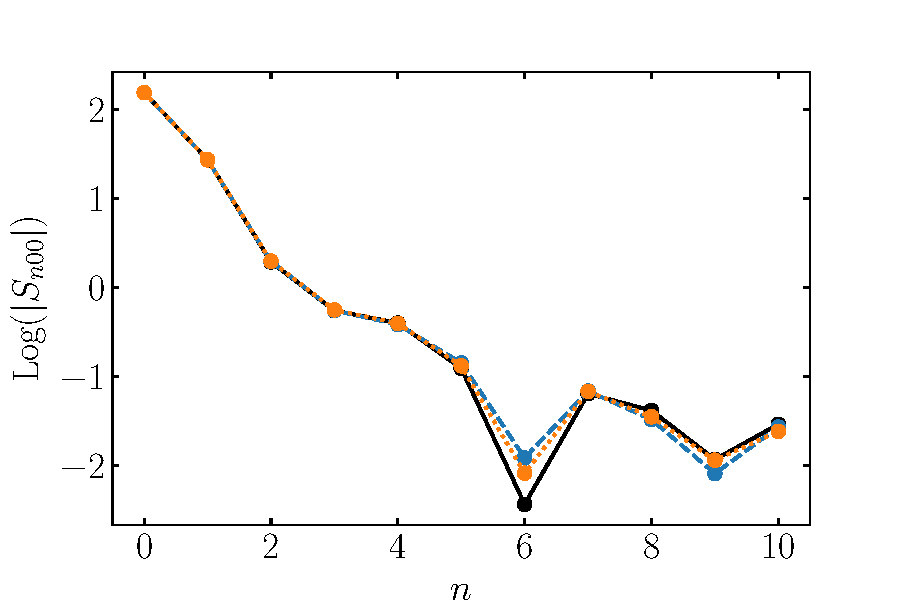
\includegraphics[scale=0.5]{../code/S_n_henrquist.pdf}
  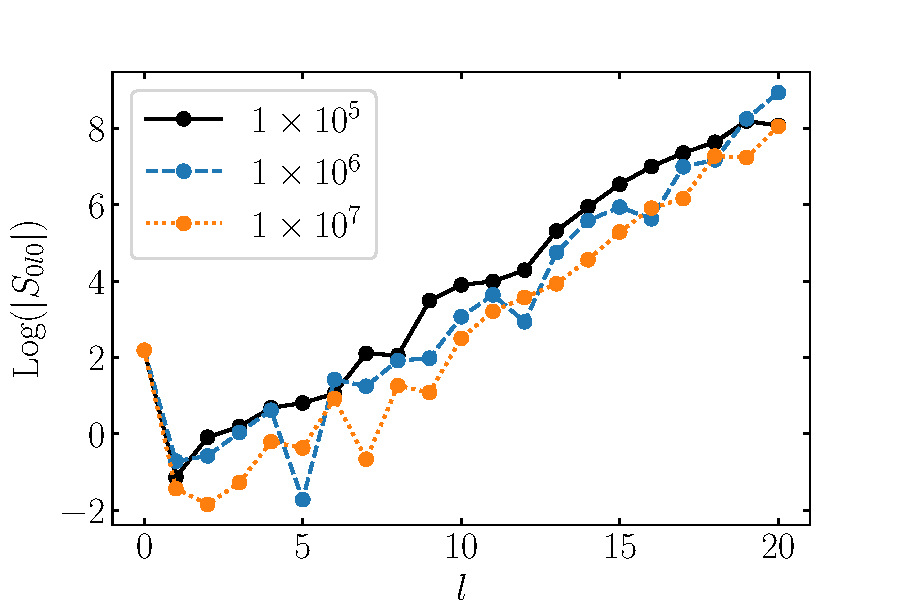
\includegraphics[scale=0.5]{../code/S_l_henrquist.pdf}
  \caption{Coefficients computed using equation \label{eq:coeff} as a function
  of $n$ (left) and $l$ (right) for three different resolutions. The amplitude of the coefficients increase
  exponentially with $l$} \label{fig:coeff_hernquist}
\end{figure}


\begin{figure}[H]
  \centering
  %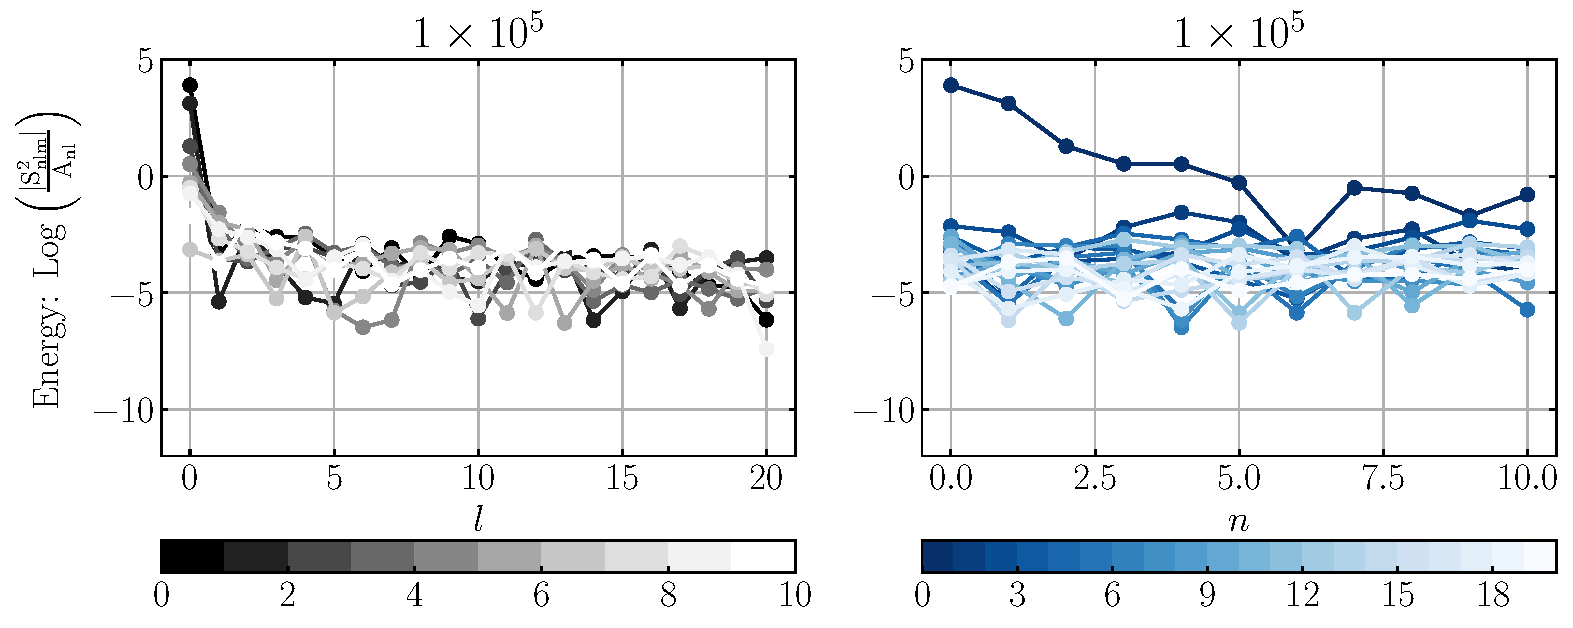
\includegraphics[scale=0.5]{../code/energy_terms_hern_a_40_1E5.pdf}
  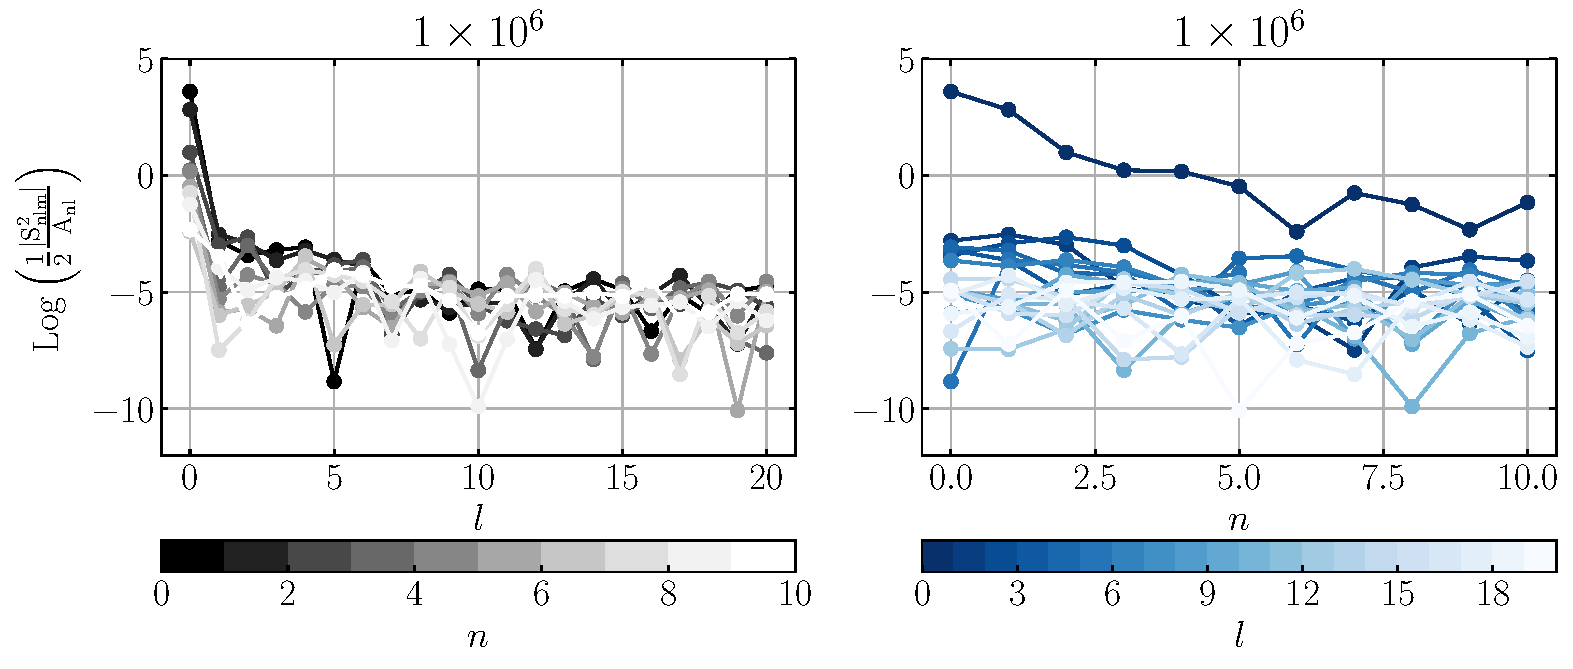
\includegraphics[scale=0.5]{../code/energy_terms_hern_a_40_1E6.pdf}
  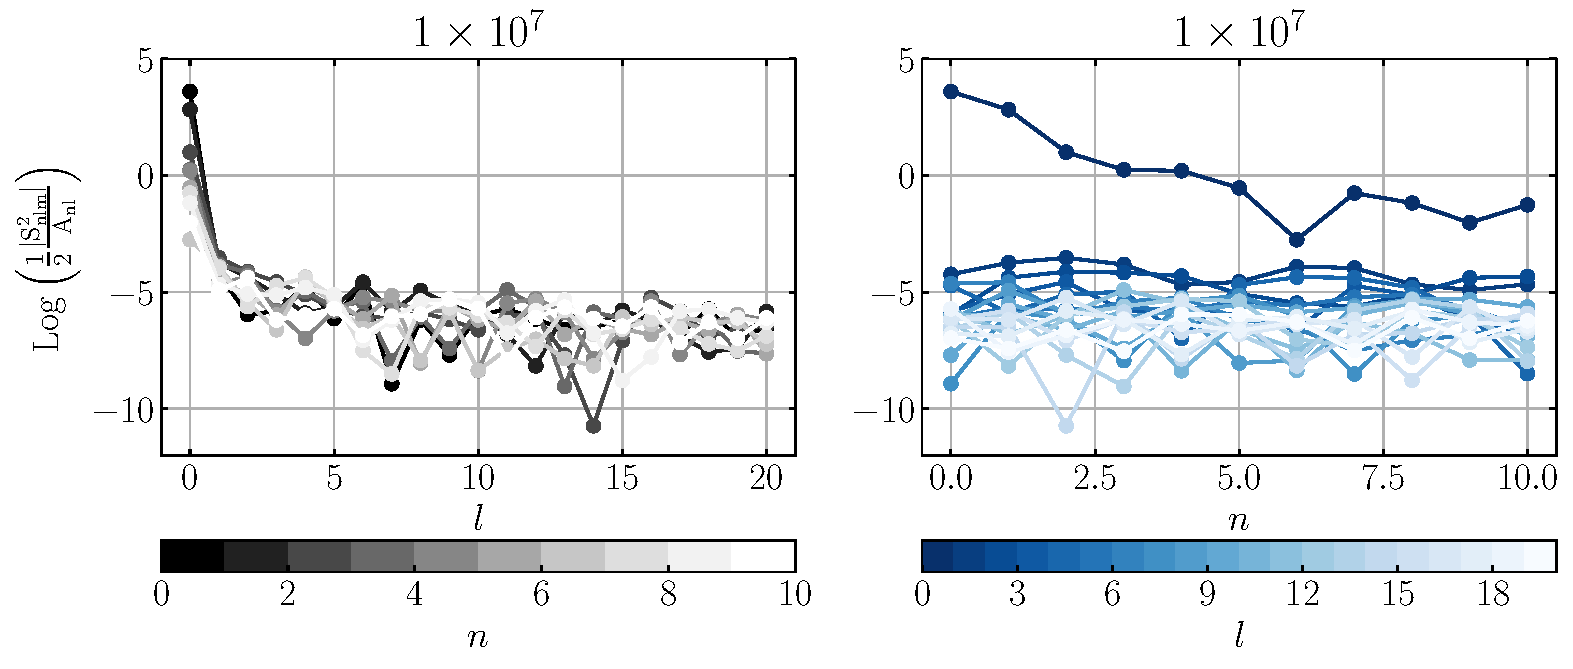
\includegraphics[scale=0.5]{../code/energy_terms_hern_a_40_1E7.pdf}
  \caption{Terms on the potential energy as defined in equation 
  \ref{eq:energy} for a Hernquist spherical halo. On the left panel the dependency on $l$ is shown for every value of $n$ color lines. 
On the right the dependency on $n$ is shown for every value of $l$. Each row represent a halo with different number of particles, the highest resolution halo is on the bottom. Only the coefficients 
with $n<6$ and $l=0$ have values larger than 0. As the resolution of the halos increases the amplitudes 
of the 'energies' for those coefficients with $l>0$.}\label{fig:spherical_energy}
\end{figure}

\subsection{Oblate halo}

If one repeats the computations of the coefficients and the energy terms for a
Hernquist \textit{oblate} halo with axis ratios of 1.8 one finds that the coefficients
with $l=2,4,6$ have higher amplitudes when compare to the spherical case as shown
in Figure \ref{fig:oblate_coeff}. 


\begin{figure}[H]
  \centering
  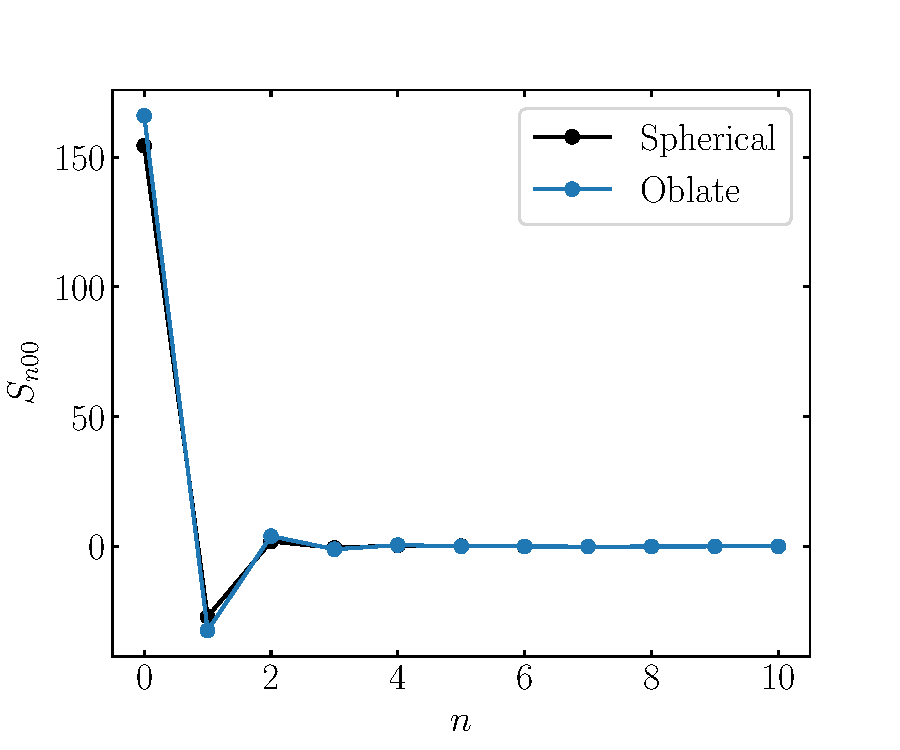
\includegraphics[scale=0.5]{../code/S_n_henrquist_oblate.pdf}
  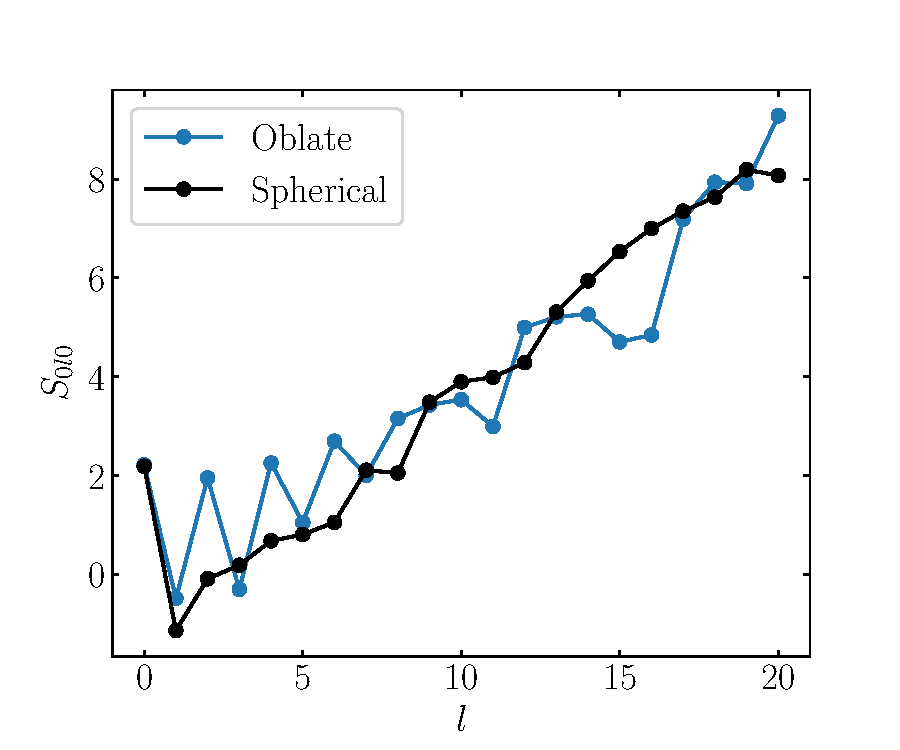
\includegraphics[scale=0.5]{../code/S_l_henrquist_oblate.pdf}
  \caption{Expansion coefficients computed using equation \label{eq:coeff} for 
  a Hernquist oblate halo with axis ratio of 1.8 (Blue lines) for comparison the 
    coefficients for a spherical Hernquist halo are shown in Black line. For the
oblate halo, the coefficients with $l=m=0$ (left panel) have the same amplitudes as in the
spherical halo. However, coefficients with $l>0$ (right panel) have larger amplitudes 
than those for the spherical halo, specially those with $l=2,4,8$. The amplitude increases with $l$ as in the spherical case.} \label{fig:oblate_coeff}
\end{figure}

The corresponding energy terms are shown in Figure \ref{fig:energy_oblate}

\begin{figure}[H]
  \centering
  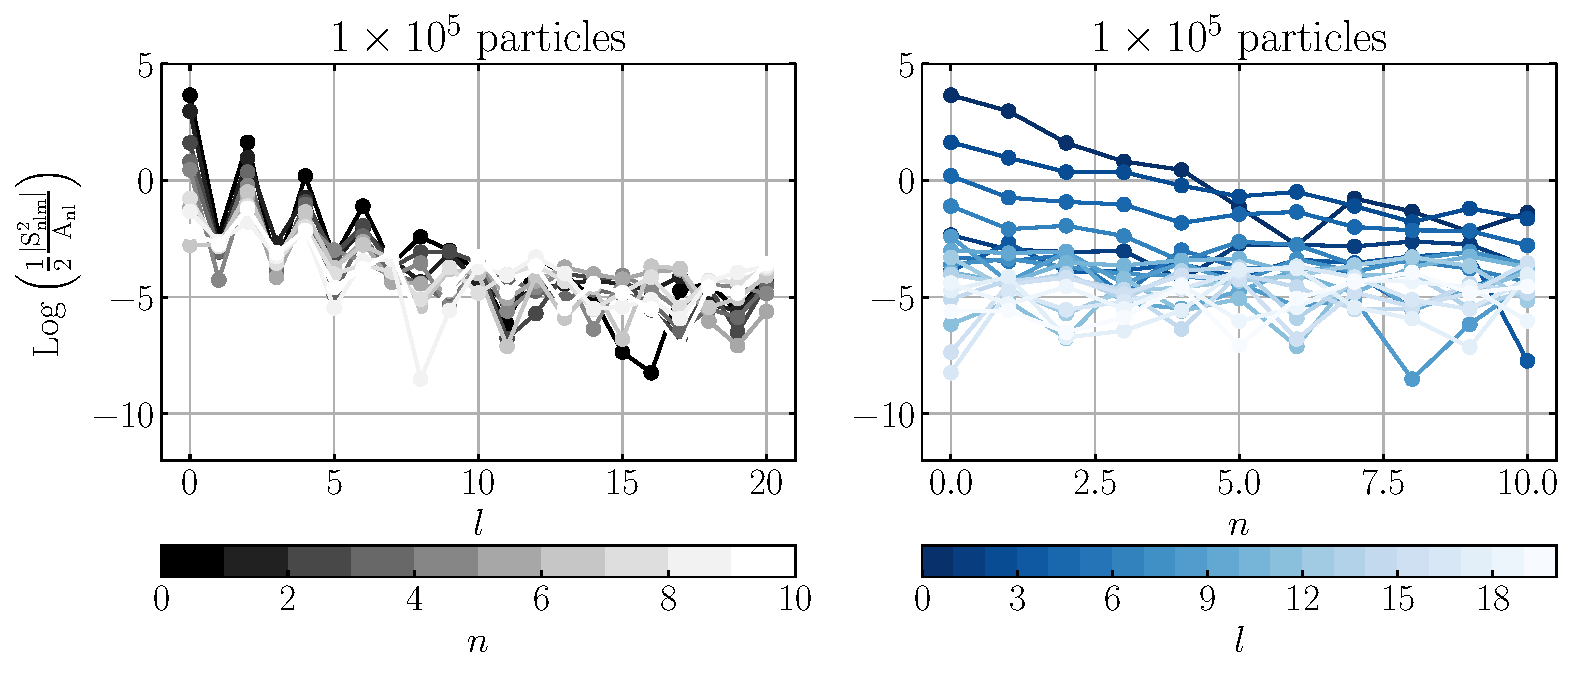
\includegraphics[scale=0.5]{../code/energy_terms_oblate_hern_a_40_1E5.pdf}
  \caption{Terms on the potential energy contribution for the oblate Hernquist halo.
The amplitude of the terms with l=[2, 4] is larger than 0.} \label{fig:energy_oblate}
\end{figure}




\textbf{Conclusion:} The coefficients naturally increase as a function of $l$
even if the underlying halo is is Hernquist halo. However, the amplitude of those terms
to the 'energy' is small as shown in the right panel of Figure \ref{fig:spherical_energy}.\\



\section{BFE applied to a MW-like galaxy in isolation (no LMC).}

\textbf{Strategy:}\\

\begin{enumerate}
  \item Compute the coefficients of the BFE on the DM particles of the MW using
    snapshots with different resolutions.
  \item Compute the accelerations of the MW DM halo particles using the BFE.
  \item Compute the accelerations of the MW DM halo particles using
    \verb+gadget+ particles.

  \item Compare the value of the acceleration obtain with the BFE and with
    Gadget.
  \item Use the energy of the coefficients to select the most `energetic' coefficients to study how
    the acceleration computation will deviate when changing the number of
    coefficients in the BFE.
\end{enumerate}



\subsection{Potential profile:}


\begin{figure}[H]
  \centering
  \includegraphics[scale=0.7]{../../MW-LMC-SCF/code/pot_iso_mw.pdf}
  \caption{\textit{Upper:} Potential computed with Gadget (solid color lines)
  and the BFE (black dashed line) for a MW-like halo with three different
  resolutions corresponding to $10^6, 10^7, 10^8$ DM particles. For the BFE the
  potential was computed using coefficients up to order
  $n=20$, $l=20$ and $m=20$ in the lowest resolution DM halo. \textit{Bottom:}
  Percentage difference between the potential computed with Gadget and the BFE.
  In each chase, the BFE is computed with the corresponding DM halo resolution
  using only the 1st coefficient ($n=0$, $l=0$, $m=0$) given that it is
  the most energetic. \textbf{The main different is in the outskirts of the
  halo, not sure yet why this is happening.}}
\end{figure}


\subsection{Acceleration:}


\begin{figure}[H]
  \centering
  \includegraphics[scale=0.65]{../../MW-LMC-SCF/code/mw_iso_acc.pdf}
  \caption{\textit{Upper:} Percentage difference in the acceleration computed with Gadget 
  and the BFE for three MW-like halo with three different
  resolution corresponding to $10^6, 10^7, 10^8$ DM particles. For the BFE, the
  potential was computed using coefficients up to order
  $n=20$, $l=20$ and $m=20$ at every resolution.
  \textit{Bottom:}
  Histogram of the percentage difference between the acceleration computed with Gadget and the BFE.
  In each chase the BFE is computed with the corresponding DM halo resolution
  using only the 1st coefficient ($n=0$, $l=0$, $m=0$) given that it is
  the most energetic.}
\end{figure}



\section{BFE applied to the MW+LMC simulation}

In this section, the coefficients in the BFE for the simulation with the MW and
the LMC are computed as shown in Figure \ref{fig:MW_LMC_coeff}.

\begin{figure}[H]
  \centering
  \includegraphics[scale=0.5]{../../MW-LMC-SCF/code/MWLMC_S_coeff_energy.pdf}
  \caption{Gravitational potential energy of the coefficients as a function of
  $l$ (left panel) and $n$ (right panel). There
  is not clear signal of an oblate or prolate halo.}\label{fig:MW_LMC_coeff}
\end{figure}


\subsection{BFE potential, density and acceleration}


\begin{figure}[H]
  \centering
  \includegraphics[scale=0.5]{../../MW-LMC-SCF/code/BFE_potential.pdf}
  \includegraphics[scale=0.5]{../../MW-LMC-SCF/code/BFE_density.pdf}
  \caption{Slices in the $y$-$z$ plane of the density (Top panels) 
  and the potential (Bottom panels) computed with the BFE. The
  left column shows the potential and density using all the coefficients
  in the BFE (9261 coefficients). The middle column shows the density and potential from the
  first coefficient ($n=0$, $l=0$ and $m=0$). The right column shows the
  density and potential contrasts $\Delta \rho$ and $\Delta \Phi$. The
  structure of the wake is reveal in the density contrast.}

\end{figure}



\begin{figure}[H]
  \centering
  \includegraphics[scale=0.5]{../../MW-LMC-SCF/code/accelerations_BFE_MWLMC.pdf}
  \caption{Slice in the $y$-$z$ plane of the accelerations in each component.
  $a_x$ top, $a_y$ middle and $a_z$ bottom. The left column shows the
  acceleration computed with all the coefficients in the BFE. The acceleration
  is mainly in the $a_x$ component since this component is perpendicular to the
  $y_z$ plane. The structure of the wake is clearly seen in this acceleration
  component. Note, the existence of a `boundary' with very low acceleration
  values shown in purple. The middle column shows the contribution of the first
  coefficient \textbf{Why does it have this shape?}. On the right column the
  difference in the acceleration between the expansion with all the coefficients
  and the first coefficient is shown. Again, the structure of the wake is reveal 
  as negative values of in $a_x$. DM particles in the wake are accelerating
  towards the center of the MW.}
\end{figure}



\begin{figure}[H]
 \centering
 \includegraphics[scale=0.4]{../../MW-LMC-SCF/code/BFE_density_N_coeff_4_zero.png}
 \includegraphics[scale=0.4]{../../MW-LMC-SCF/code/BFE_density_N_coeff_9_zero.png}
 \includegraphics[scale=0.4]{../../MW-LMC-SCF/code/BFE_density_N_coeff_26_zero.png}
  \includegraphics[scale=0.4]{../../MW-LMC-SCF/code/BFE_density_N_coeff_62_zero.png}
  \includegraphics[scale=0.4]{../../MW-LMC-SCF/code/BFE_density_N_coeff_136_zero.png}
  \includegraphics[scale=0.4]{../../MW-LMC-SCF/code/BFE_density_N_coeff_266_zero.png}
  \includegraphics[scale=0.4]{../../MW-LMC-SCF/code/BFE_density_N_coeff_606_zero.png}
  \includegraphics[scale=0.4]{../../MW-LMC-SCF/code/BFE_density_N_coeff_2485_zero.png}
  \caption{Relative density $\Delta \rho=\frac{\rho_{nlm}}{\rho_{000}}-1) $surfaces computed with the BFE coefficients selected with
  different `Energy' cuts relative to the density from the first coefficients
  i.e $S_{000}$. The DM wake can be seen when more than 26 coefficients are
  used.}
\end{figure}




%\begin{figure}[H]
%  \centering
%  \includegraphics[scale=0.4]{../../MW-LMC-SCF/code/BFE_density_N_coeff_20_zero.png}
%  \includegraphics[scale=0.4]{../../MW-LMC-SCF/code/BFE_density_N_coeff_24_zero.png}
%  \includegraphics[scale=0.4]{../../MW-LMC-SCF/code/BFE_density_N_coeff_28_zero.png}
%  \includegraphics[scale=0.4]{../../MW-LMC-SCF/code/BFE_density_N_coeff_33_zero.png}
%  \includegraphics[scale=0.4]{../../MW-LMC-SCF/code/BFE_density_N_coeff_37_zero.png}
%  \includegraphics[scale=0.4]{../../MW-LMC-SCF/code/BFE_density_N_coeff_42_zero.png}
%  \includegraphics[scale=0.4]{../../MW-LMC-SCF/code/BFE_density_N_coeff_46_zero.png}
%  \includegraphics[scale=0.4]{../../MW-LMC-SCF/code/BFE_density_N_coeff_51_zero.png}
%  \includegraphics[scale=0.4]{../../MW-LMC-SCF/code/BFE_density_N_coeff_55_zero.png}
%  \includegraphics[scale=0.4]{../../MW-LMC-SCF/code/BFE_density_N_coeff_60_zero.png}
%  \caption{Relative density $\Delta \rho=\frac{\rho_{nlm}}{\rho_{000}}-1) $surfaces computed with the BFE coefficients selected with
%  different `Energy' cuts relative to the density from the first coefficients
%  i.e $S_{000}$. The DM wake can be seen when more than 26 coefficients are
%  used.}
%\end{figure}





%\begin{figure}[H]
%  \centering
%  \includegraphics[scale=0.55]{../../MW-LMC-SCF/code/pot_convergence.pdf}
%  \caption{Percentage error between the BFE potential computed with all the
%  coefficients and the potential computed using coefficients above an energy
%  threshold. On the x-axis the energy threshold is shown. As the coefficients with
%  lower energy are included the percentage error decreases. Errors below 1\% are
%  found for coefficients of order larger than $n=3, l=0, m=0$}
%\end{figure}




%\begin{figure}[H]
%  \includegraphics[scale=0.55]{../../MW-LMC-SCF/code/a_convergence.pdf}
%  \caption{Percentage error between the BFE acceleration computed with all the
%  coefficients and the acceleration computed using coefficients above an energy
%  threshold. On the x-axis the energy threshold is shown. Errors below 1\% are
%  found for coefficients or order larger than $n=20, l=7, m=6$}
%\end{figure}



%\begin{figure}[H]
%  \centering
%  \includegraphics[scale=0.6]{../../MW-LMC-SCF/code/gadget_bfe.png}
%  \caption{Potential of the simulation with the MW and the LMC computed with Gadget (black dots) and with the BFE (solid
%  blue line). The difference between these two is because neither the disk
%  and the bulge potential have been added to the BFE potential.}
%\end{figure}




\begin{figure}[H]
  \centering
  \includegraphics[scale=0.65]{../../MW-LMC-SCF/code/mwlmc_acc.pdf}
  \caption{Difference in the acceleration computed with the BFE and Gadget. On
  the top panel the percentage difference is shown for halos with different
  resoluion. For the low res halo (black dots) the BFE do not reproduce
  accurately the accelration computed with Gadget in the outskirts of the halo.
  On the bottom panel a histogram of the acuracy of the the particles is
  summarized. The BFE is more accurate for the High resolution halo.}
\end{figure}


\begin{figure}[H]
  \centering
  \includegraphics[scale=0.55]{../../MW-LMC-SCF/code/mwlmc_acc_nlm_3.pdf}
  \includegraphics[scale=0.55]{../../MW-LMC-SCF/code/mwlmc_acc_nlm_2.pdf}
  \includegraphics[scale=0.55]{../../MW-LMC-SCF/code/mwlmc_acc_nlm_1.pdf}
  \includegraphics[scale=0.55]{../../MW-LMC-SCF/code/mwlmc_acc_nlm_0.pdf}
  \caption{Histogram of the accuracies in the accelerations as a function of the
  number of coefficients (shown in the different panels).}
\end{figure}



\subsection{Optimal convergence using the signal to noise of the coefficients:}

\subsubsection{Computing the signal to noise of the coefficients:}


\begin{equation}
  var(\hat{a}_j) = \dfrac{1}{N}{E[\Psi_j\Psi_j] - E[\Psi_j]E[\Psi_j]}
\end{equation}

Which in Lowing (2011) notation would be:

\begin{equation}\label{eq:var}
  var(S_{n,l,m}) = m \left[ \sum_{i}^{N}m_i \Psi_{n,l,m}^2(x_i)
   - \left(\sum_{i}^{N}m_i \Psi_{n,l,m}(x_i)\right)^2
   \right]
\end{equation}

The first term in the right hand side is the covariance matrix and
the second term of Eq.\ref{eq:var} are the coefficients
$\hat{S}_{n,l,m}^2$ and $\hat{T}_{n,l,m}^2$. $m$ is the particle
mass and $\Psi_{nlm}$ is defined as:

\begin{equation}
  \Psi_{nlm}(x_i) = (2-\delta_{m,0})
  \tilde{A}_{n,l}\Phi_{n,l}(r_i)Y_{l,m}(\theta_i)cos(m\phi_i)
\end{equation}

The covariance matrix in the Lowing (2011) notation takes the form:

\begin{equation}
  \tilde{S}_{nlm n'l'm'} = \hat{S}_{nlm} \hat{S}_{n'l'm'}
\end{equation}

The smoothening of the coefficients is computed as follows:

\begin{equation}
  bS_{nlm} = \dfrac{1}{1 + var(\hat{S}_{nlm})/{S_{nlm}}^2}
\end{equation}

\begin{equation}
  bT_{nlm} = \dfrac{1}{1 + var(\hat{T}_{nlm})/{T_{nlm}}^2}
\end{equation}



\subsubsection{Results:}

Computed and tested with \verb+Gala+ and a parallel  C code written by me. 


\begin{figure}[H]
  \centering
  \includegraphics[scale=0.5]{../../MW-LMC-SCF/code/energies_smoothed_n_0.pdf}
  \caption{Comparison of the smoothed and non-smoothed terms (right panels). On the top left
  panel the difference in the energies between the smoothed and non-smoothed
  coefficients are shown. On the bottom left panel the value of $b$ is shown.}
\end{figure}


\begin{figure}[H]
  \centering
  \includegraphics[scale=0.6]{../../MW-LMC-SCF/code/smoothing.pdf}
  \caption{Signal to noise computed using each coefficient variance for the
  $S_{nlm}$ (left) and $T_{nlm}$ (right) coefficients. The horizontal lines
  denote when the signal to noise is 1 (dashed line) and the suggested value of
  0.3 by Weinberg (1996) (solid line). The number of coefficients could also be
  picked if a cut in $b$ is made. For example, there are 6934 of 9261 coefficients with
  $bS_{nlm}<0.3$ and 7109 of 9261 with $bT_{nlm}$}
\end{figure}



\begin{figure}[H]
  \centering
  \includegraphics[scale=0.6]{../../MW-LMC-SCF/code/delta_a_ncoeff.pdf}
  \caption{Difference in the accelerations using the smoothed (left panel) and
  non-smoothed coefficients. }
\end{figure}



\subsubsection{Comparison with the cuts in energies.}

Are the most smoothed terms related with the less energetic terms? 


\begin{figure}[H]
  \centering
  \includegraphics[scale=0.7]{../../MW-LMC-SCF/code/common_coeff.pdf}
  \caption{Fraction of coefficients that are common when doing cuts in energy
  and with the smoothing.}
\end{figure}



\begin{figure}[H]
  \centering
  \includegraphics[scale=0.7]{../../MW-LMC-SCF/code/delta_a_gadget_dif_res.pdf}
  \includegraphics[scale=0.7]{../../MW-LMC-SCF/code/delta_a_bfe_dif_res.pdf}
  \includegraphics[scale=0.7]{../../MW-LMC-SCF/code/delta_a_gadget_bfe_dif_res.pdf}
  \caption{Percentage difference between the acceleration $\Delta a$ computed using
  different resolution halos. On the top panel $\Delta a$ is shown for the
  acceleration computed with Gadget for halos with different resolutions. On the
  middle panel $\Delta a$ is shown for the acceleration computed with the BFE.
  On the bottom panel the differences between Gadget and BFE is shown. The
  differences in the acceleration as a function of halo resolution is larger
  in Gadget than using the BFE.}
\end{figure}



\begin{figure}[H]
  \centering
  \includegraphics[scale=0.7]{../../MW-LMC-SCF/code/a_disp_bfe_gadget_dif_res.pdf}
\end{figure}

\begin{figure}[H]
  \centering
  \includegraphics[scale=0.7]{../../MW-LMC-SCF/code/da_vs_smoothing.pdf}
\end{figure}

\textbf{To-do:}\\




\begin{itemize}
  
  \item Discuss how to choose the number of coefficients.
  \item Should we try smoothing the density in the low res halo to see if the
    BFE can do better? 
  \item Include the LMC potential. Apply the BFE to the LMC.
\end{itemize}


\subsection{Fun plots}



\begin{figure}[H]
  \centering
  \includegraphics[scale=0.5]{../../MW-LMC-SCF/code/potential_of_low_u_terms.pdf}
  \includegraphics[scale=0.5]{../../MW-LMC-SCF/code/density_of_low_u_terms.pdf}
  \caption{Potential (left panel) and density (right panel) of the lowest energy terms.}
\end{figure}


\bibliography{references}


\appendix


\section*{Appendix: A review of the BFE formalism:}\label{sec:appendix}

In this document we will follow the notation presented \cite{Lowing11}. Table
\ref{tab:conversion} shows the conversion between the notation used in \cite{Hernquist92} and
in \cite{Lowing11}.

\begin{table}[h]
  \centering
  \begin{tabular}{c  c}
    \hline
    \hline
    \cite{Hernquist92} notation & \cite{Lowing11} notation \\
    \hline
    $A_{nlm}$ & $S_{nlm} cos\ m\phi + T_{nlm}sin\ m\phi $\\
    $I_{nl} = \frac{1}{\tilde{A}_{nl}}$ & $\frac{1}{\tilde{A}_{nl}}$\\
    $K_{nl}$ & $K_{nl}$ \\
    $\tilde{\rho}_{nl}$ & $\rho_{nl}$\\
    $\tilde{\Phi}_{nl}$ & $\Phi_{nl}$\\
    \hline
    \hline
  \end{tabular}
  \caption{Notation conversion between \cite{Hernquist92} and the
  \cite{Lowing11} works}\label{tab:conversion}
\end{table}



The main idea of the BFE formalism is to expand the potential and density in
angular and radial functions. 


\begin{equation}
    \rho(r, \theta, \phi) = \sum_{nlm} A_{nlm}\rho_{nlm}(r, \theta, \phi)
\end{equation}

\begin{equation}
    \Phi(r, \theta, \phi) = \sum_{nlm} A_{nlm}\Phi_{nlm}(r, \theta, \phi)
\end{equation}

Where $A_{nlm}$ are the coefficients of the expansion. The angular and radial
dependencies can be separated follows:


\begin{equation}\label{eq:potdens_nlm}
  \begin{aligned}
  \Phi_{nlm}(r, \theta, \phi) = \Phi_{nl}(r)Y_{lm}(\theta, \phi)\\ 
  \rho_{nlm}(r, \theta, \phi) = \rho_{nl}(r)Y_{lm}(\theta, \phi) 
  \end{aligned}
\end{equation}


Where $Y_{lm}(\theta,\phi)$ are the spherical harmonics. The radial component
is expended around a Hernquist profile multiplied by the Ultraspherical
polynomials $C_{n}(\xi)$.


\begin{equation}
  \Phi_{nl}(r) = - \dfrac{r^l}{r(1+r)^{2l+3}}C_{n}^{2l+3/2}(\xi)\sqrt{4\pi}
\end{equation}

\begin{equation}
  \rho_{nl}(r) = \dfrac{K_{nl}}{2\pi}\dfrac{r^l}{(1+r)^{2l+1}}C_{n}^{2l+3/2}(\xi)\sqrt{4\pi}
\end{equation}


Where $K_{nl}$ is defined as:

\begin{equation}
    K_{nl}=\dfrac{1}{2}n(n+4l+3) +(l+1)(2l+1)
\end{equation}

The real form of equation \ref{eq:potdens_nlm} takes the form: 

\begin{equation}
  \rho(r, \theta, \phi) = \sum_{n} \sum_l \sum_m Y_{lm}(\theta) \rho_{nl}(r)
  \left[ S_{nlm} cos\ m \phi + T_{nlm} sin m\ \phi \right]
\end{equation}


\begin{equation}
  \Phi(r, \theta, \phi) = \sum_{n} \sum_l \sum_m Y_{lm}(\theta) \Phi_{nl}(r)
  \left[ S_{nlm} cos\ m\phi + T_{nlm} sin\ m \phi \right]
\end{equation}


The coefficients can be computed using the orthonormal properties of the
Spherical harmonics and the Ultraspherical polynomials this is:

\begin{equation}\label{eq:energy}
  I_{nlm}^{n'l'm'} = \int_V \rho_{nlm} \Phi_{n'l'm'}^*  d\textbf{r} = \tilde{A}_{nl} \delta_{nn'}
  \delta_{ll'} \delta_{mm'} 
\end{equation}

Where $\tilde{A}_{nl}$ is found to be:

\begin{equation}
    \tilde{A}_{nl} = - \frac{1}{K_{nl}}\frac{2^{8l+6}}{4\pi}\frac{n!(n+2l+3/2)[\Gamma(2l+3/2)]^2}{\Gamma(n+4l+3)}
\end{equation}

With these relations the coefficients can be derived as follows:

\begin{equation}\label{eq:coefficients}
  I_{nlm} = \int_V \rho(r) \Phi_{nlm} d\textbf{r} = 
\end{equation}


\begin{equation}
  \begin{aligned}
    S_{nlm} = (2-\delta_{m0})\tilde{A}_{nl} \sum_k m_k
  \Phi_{nl}(r_k)Y_{lm}(\theta_k) cos\ m\phi_k \\
    T_{nlm} = (2-\delta_{m0})\tilde{A}_{nl} \sum_k m_k 
  \Phi_{nl}(r_k)Y_{lm}(\theta_k) sin\ m\phi_k 
  \end{aligned}
\end{equation}


With these results we can compute the total gravitational energy of the system
as:

\begin{equation}
  U = \dfrac{1}{2} \int_V \rho(r)\Phi(r)^{*} = \int_v  \sum_{nlm} A_{nlm}^2 \rho_{nlm}(r,
  \theta, \phi) \phi_{nlm}(r, \theta, \phi) = \sum_{nlm}
  \frac{A_{n'l'm'}^2}{\tilde{A}_{nl}}
  \delta_{nn'}\delta_{ll'}\delta_{mm'} 
\end{equation}

\begin{equation}
  U = \dfrac{1}{2}\sum_{nlm} \frac{A_{n'l'm'}^2}{\tilde{A}_{n'l'}} = \sum_{nlm} U_{n'l'm'}
\end{equation}




\end{document}
